\documentclass[a4paper,12pt]{article} %размер бумаги устанавливаем А4, шрифт 12пунктов
%\usepackage[T2A]{fontenc}
\usepackage[utf8]{inputenc}
\usepackage{csquotes}
\usepackage[english,russian]{babel}%используем русский и английский языки с переносами
\usepackage{biblatex}
\bibliography{refs}
\usepackage{amssymb,amsfonts,mathtext,enumerate,float} %подключаем нужные пакеты расширений
\usepackage{textcomp}
\usepackage{adjustbox}
\usepackage{graphicx} %хотим вставлять в диплом рисунки?
%\graphicspath{{images/}}%путь к рисункам
\makeatletter
\makeatother
\usepackage{sagetex}
\usepackage{geometry} % Меняем поля страницы
\geometry{left=2cm}% левое поле
\geometry{right=1.5cm}% правое поле
\geometry{top=1cm}% верхнее поле
\geometry{bottom=2cm}% нижнее поле




%\usepackage{tabularx} 

\usepackage{epstopdf}
\usepackage{amsmath} %отображение математической нотации
\usepackage{caption, subcaption} %подписи}
\usepackage{indentfirst}%отступ вначале параграфа
\usepackage{pscyr}
%\usepackage{natbib}
%\usepackage{ragged2e} %для таблиц
 
\captionsetup[table]{labelsep = endash, singlelinecheck=false}
\captionsetup[figure]{name = Рисунок, labelformat=simple, labelsep = endash}

\begin{document}


\newcommand\tline[2]{$\underset{\text{#1}}{\text{\underline{\hspace{#2}}}}$}
\newcommand\nameLine[3]{$\underset{\text{#1}}{\text{\underline{\text{#2}\hspace{#3}}}}$}

\begin{titlepage}
	\centering
	{\fontsize{12pt}{5cm}\selectfont \bfseries Министерство образования и науки Российской Федерации} \\ \vspace{0.5cm}
	{\fontsize{7pt}{5cm}\selectfont ФЕДЕРАЛЬНОЕ ГОСУДАРСТВЕННОЕ АВТОНОМНОЕ ОБРАЗОВАТЕЛЬНОЕ УЧРЕЖДЕНИЕ ВЫСШЕГО ПРОФЕССИОНАЛЬНОГО ОБРАЗОВАНИЯ} \\ 
	\vspace{1cm}
	{\fontsize{12pt}{5cm}\selectfont \bfseries САНКТ-ПЕТЕРБУРГСКИЙ УНИВЕРСИТЕТ ИНФОРМАЦИОННЫХ ТЕХНОЛОГИЙ, МЕХАНИКИ И ОПТИКИ} \\ \vspace{1.5cm}
	
	{\fontsize{14pt}{5cm}\selectfont Кафедра \hspace{1cm} \underline{Систем Управления и Информатики}  \hspace{1cm} Группа \underline{Р3340}} \\
	
	\vspace{2cm}
	
	{\fontsize{20pt}{5cm}\selectfont \bfseries Лабораторная работа №9} \\
	{\fontsize{20pt}{5cm}\selectfont \bfseries “Экспериментальное построение частотных характеристик типовых динамических звеньев”} \\
	\vspace{0.2cm}
	{\fontsize{14pt}{5cm}\selectfont Вариант - 10} \\
	
	\vspace{1.5cm}
	
	\flushleft
	{Выполнилa \hspace{1.8cm} \nameLine{(фамилия, и.о.)}{Ким А. А.}{7cm} (подпись)} \\
	
	\vspace{2cm}
	
	{Проверил \hspace{2cm} \tline{(фамилия, и.о.)}{9cm} (подпись)} \\
	
	\vspace{5cm}
	
	"\underline{\hspace{0.7cm}}"\hspace{0.2cm}\underline{\hspace{2cm}}\hspace{0.2cm}20\underline{\hspace{0.7cm}}г. \hspace{2cm} Санкт-Петербург, \hspace{2cm} 20\underline{\hspace{0.7cm}}г. \\ \vspace{1cm}
	
	Работа выполнена с оценкой \hspace{1cm} \underline{\hspace{8cm}} \\ 
	\vspace{1cm}
	Дата защиты "\underline{\hspace{0.7cm}}"\hspace{0.2cm}\underline{\hspace{2cm}}\hspace{0.2cm}20\underline{\hspace{0.7cm}}г.
\end{titlepage}

\paragraph{Цель работы:}Исследование точностных свойств систем управления.%*-без нумерации
\paragraph{Исходные данные.} В таблице 1 и таблице 2 приведены передаточная функция ОУ, характеристики задающих и возмущающих воздействий.
\begin{table}[h!]
	\caption{Исходные данные}
	\renewcommand{\arraystretch}{1.8} %строки
	%\renewcommand{\tabcolsep}{1cm} %столбцы
	\begin{tabular}{|c|c|c|c|c|c|c|c|c|}
		\hline $W_0(s)$ & $W_1(s)$ & $g = A$ & $g = Vt$ & $g = at^2/2$ &  $f_1$ & $f_2$ & Сигнал задания\\
		\hline $\displaystyle{\frac{8}{0,5s^2+2s + 8}}$& $\displaystyle{\frac{1.5s+8}{0,5s^2+2s+8}}$ & 2 & t & $0.3t^2$ & 1.5 & -0.5 & $5+t$\\
		\hline
	\end{tabular}	
\end{table}

\newpage
\begin{center}
\section{Исследование системы с астатизмом нулевого порядка}
\end{center}
\par Задана замкнутая система, структурная схема которой представлена на рисунке 1, где $H(s) = k$, $W(s)=\displaystyle{\frac{8}{0,5s^2+2s + 8}}$.
\begin{figure}[h!]
	\centering
	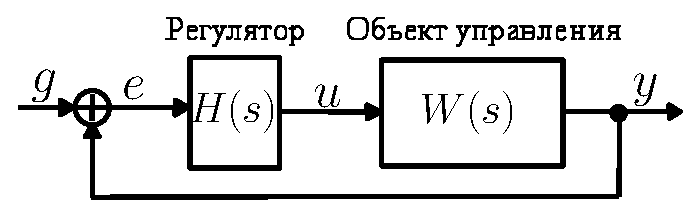
\includegraphics[width=0.5\linewidth]{scheme/scheme0.eps}
	\caption{Структурная схема моделируемой системы}
\end{figure}

\subsection{Исследование стационарного режима работы: $g(t)=A$} 
На рисунке 2 представлена структурная схема системы при входном воздействии \\$g=2$, представлены графики переходных процессов (рисунок 3) и переходные характеристики ошибок (рисунок 4) при различных значениях $k$. 
\begin{figure}[h!]
	\centering
	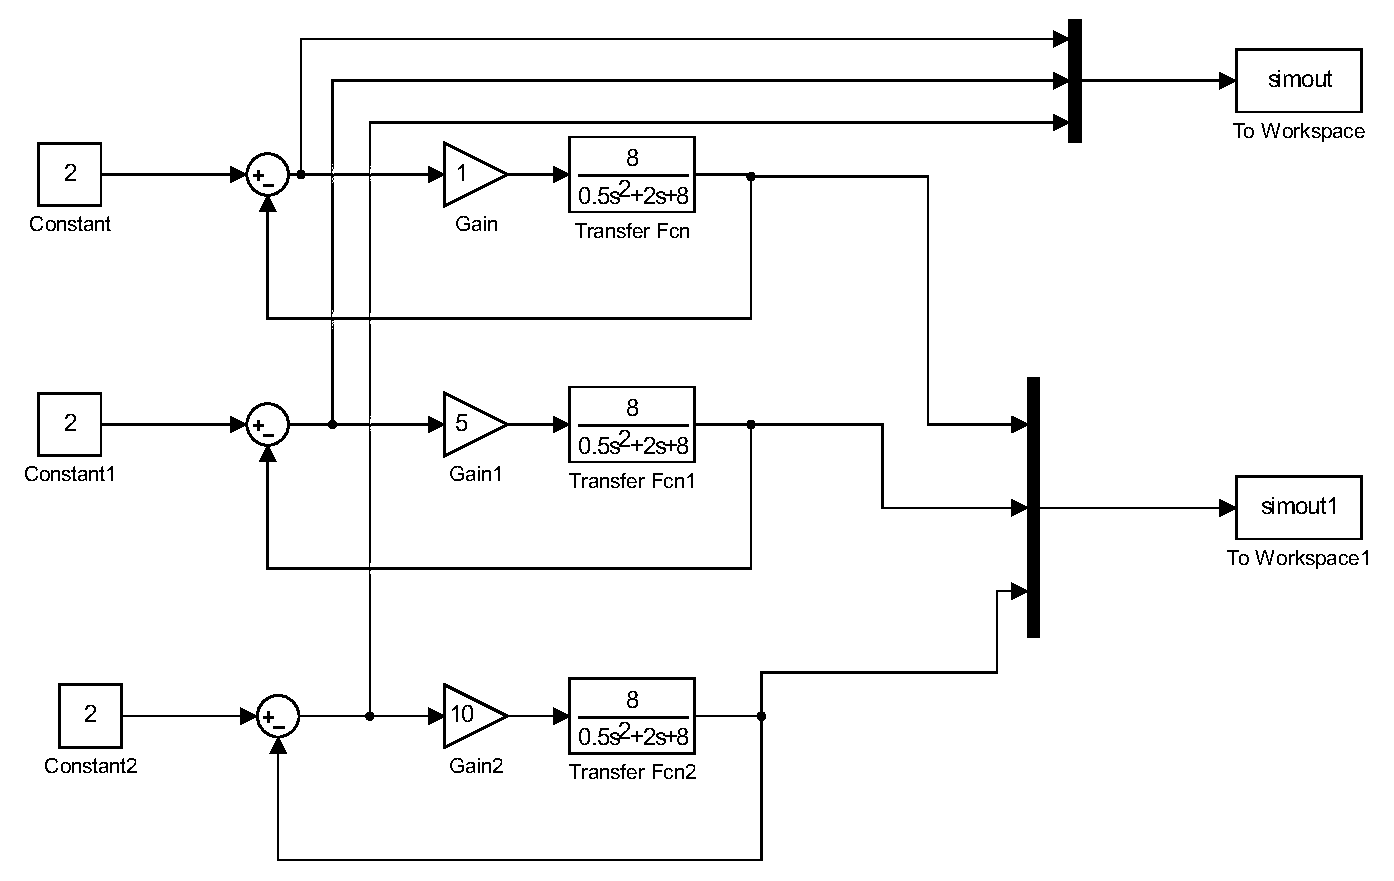
\includegraphics[width=1\linewidth]{scheme/scheme1.eps}
	\caption{Структурная схема системы с астатизмом нулевого порядка}
\end{figure}
\begin{figure}[H]
	\centering
	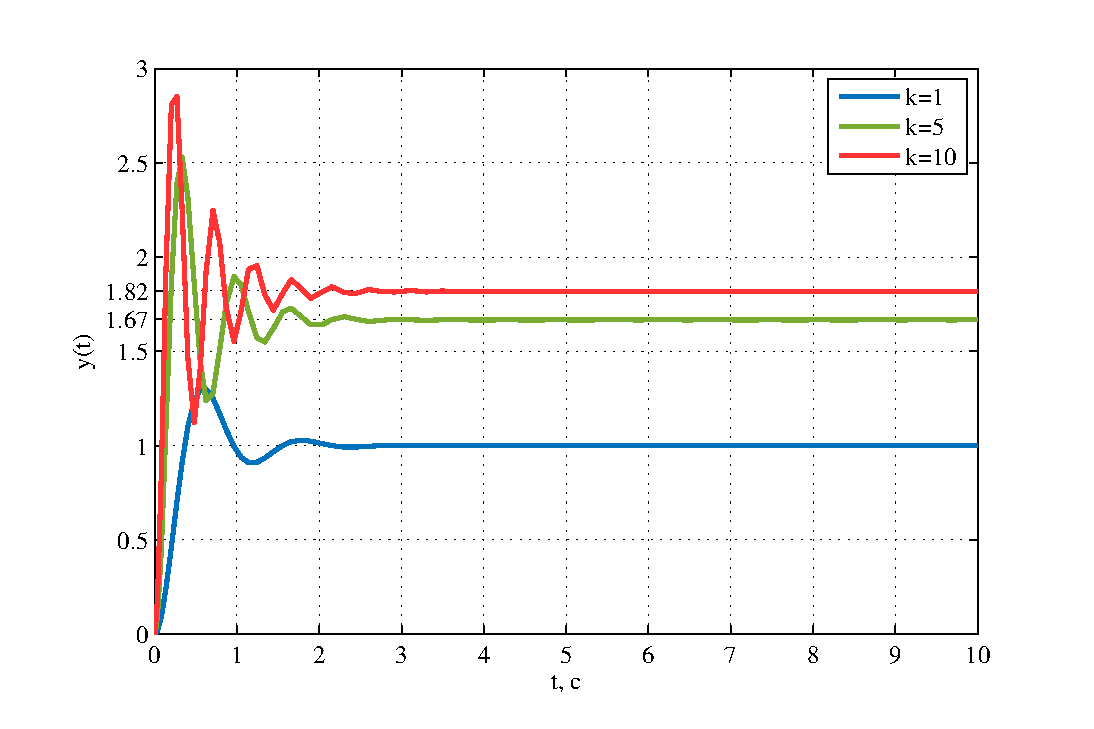
\includegraphics[width=1\linewidth]{scheme/plot1.eps}
	\caption{Переходные характеристики системы для стационарного режима работы}
\end{figure}
\begin{figure}[H]
	\centering
	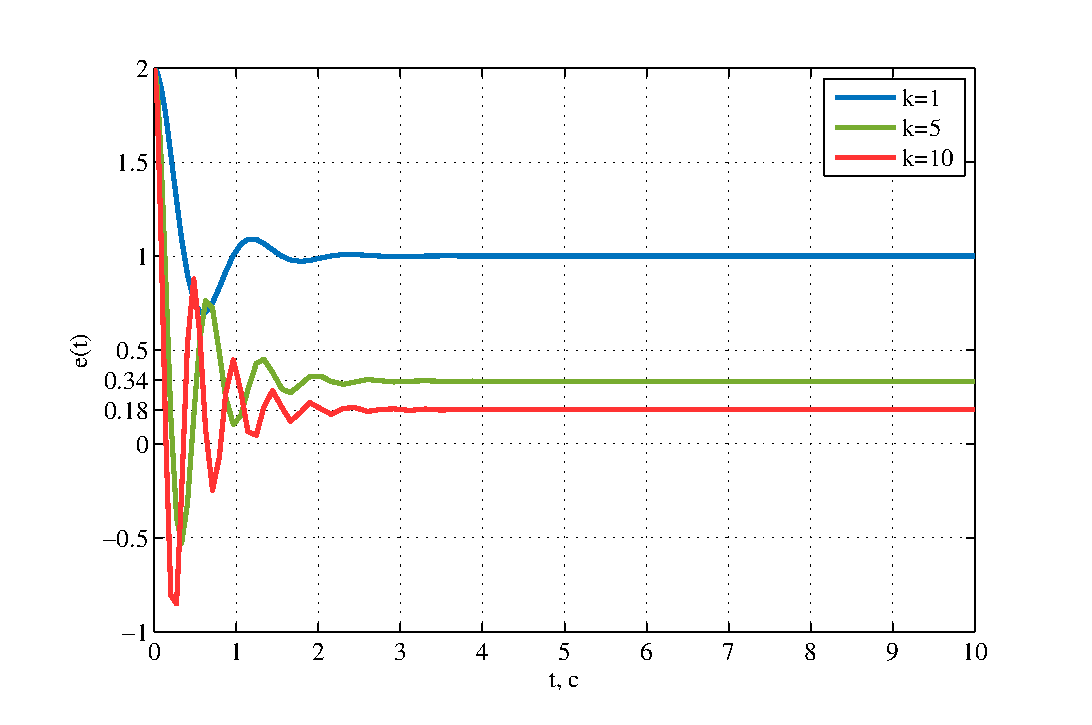
\includegraphics[width=1\linewidth]{scheme/plot2.eps}
	\caption{Переходные характеристики для ошибки}
\end{figure}
\newpage

\par С помощью расчета проверим получившееся на графике значения установившейся ошибки:
\begin{equation}
	e = \frac{A}{(1+k)}
\end{equation}
при $k=1$: $\varepsilon = \displaystyle{\frac{A}{1+k}}={\frac{2}{2}}=1;$\\
при $k=5$: $\varepsilon = \displaystyle{\frac{2}{6}}=0,33;$\\
при $k=10$: $\varepsilon = \displaystyle{\frac{2}{11}}=0,18;$\\

\subsection{Исследование режима движения с постоянной скоростью: \\$g(t)=Vt$} 
На рисунке 5 представлена переходная характеристика системы при входном воздействии $g=t$.
\begin{figure}[H]
	\centering
	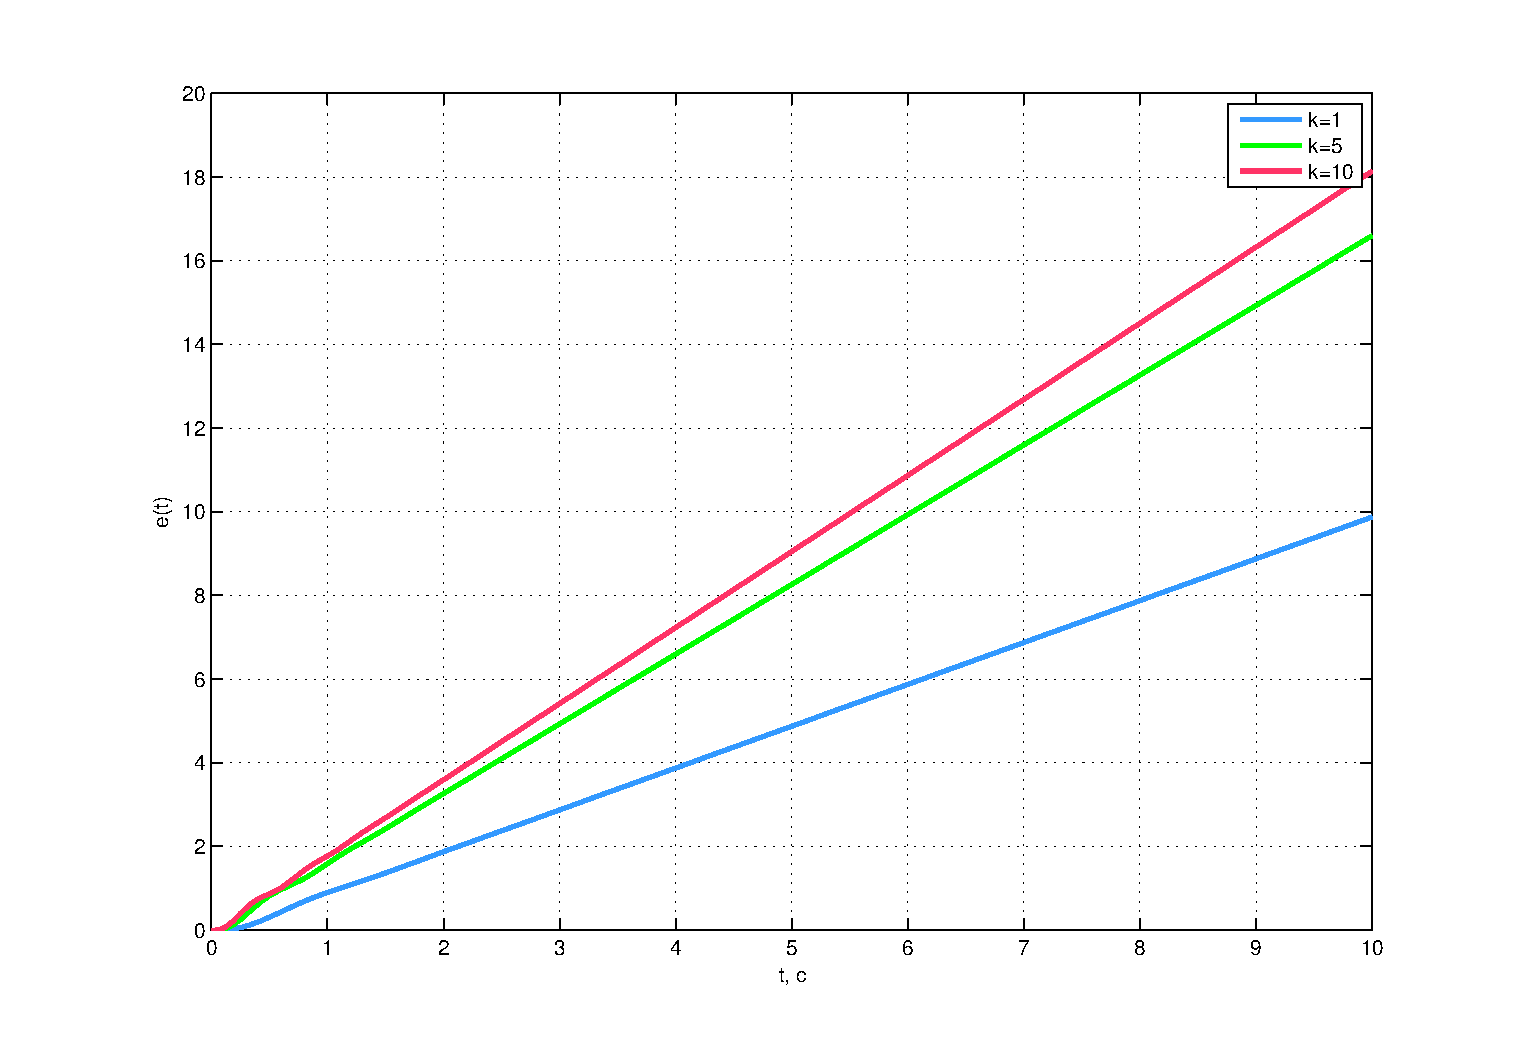
\includegraphics[width=1\linewidth]{scheme/plot3.eps}
	\caption{Переходные характеристики системы для движения с постоянной скоростью}
\end{figure}
Для статической системы при линейно нарастающем входном воздействии $g(t)=Vt$ имеем:
\begin{equation}
    \varepsilon = \lim_{s\to0} s\frac{1}{1+H(s)W(s)}G(s) = \infty.
\end{equation}\par
Вывод: в системах управления с нулевым порядком астатизма присутствует ошибка.
\newpage
\begin{center}
\section{Исследование системы с астатизмом первого порядка}
\end{center}\par
Структурная схема моделируемой системы представлена на рисунке 1, где $H(s) = \displaystyle{\frac{k}{s}},\\W(s)=\displaystyle{\frac{1.5s+8}{0,5s^2+2s+8}}$.

\subsection{Исследование стационарного режима работы: $g(t)=A$} 
На рисунке 6 представлена структурная схема системы при входном воздействии \\$g=2$, представлены графики переходных процессов (рисунок 7) и переходные характеристики ошибок (рисунок 8) при различных значениях $k$. 
\begin{figure}[H]
	\centering
	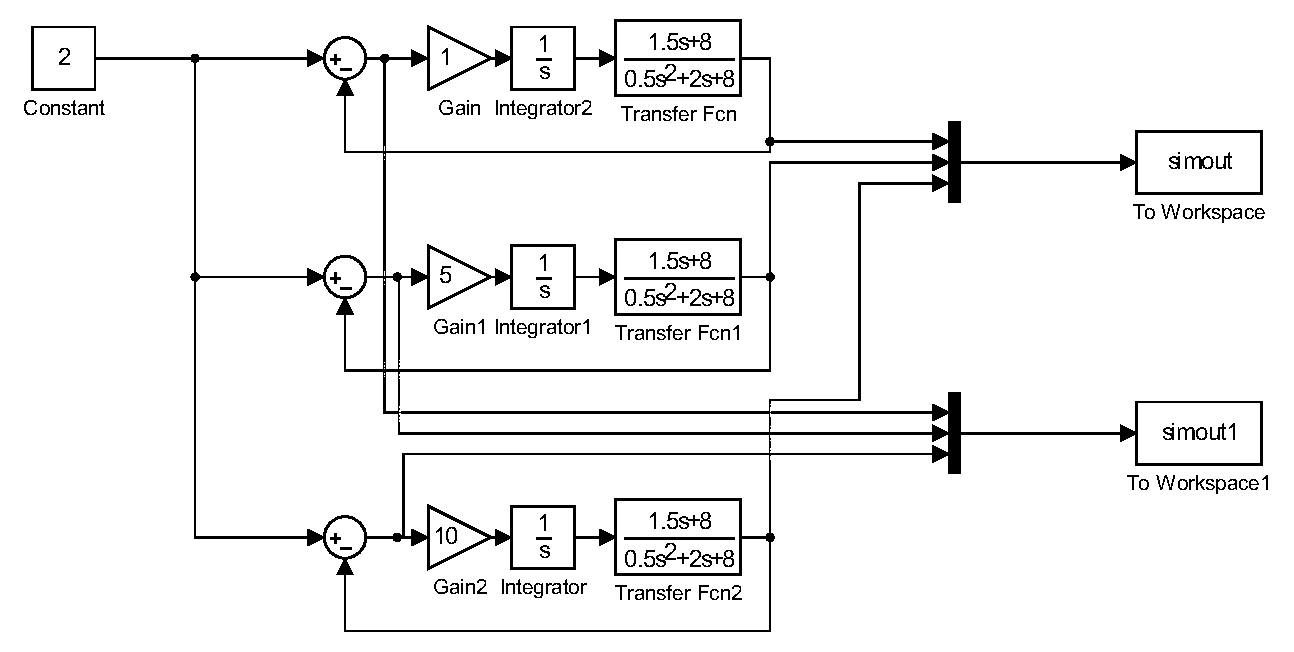
\includegraphics[width=1\linewidth]{scheme/scheme3.eps}
	\caption{Структурная схема системы с астатизмом моделируемой системы}
\end{figure}
Для статической системы при постоянном входном воздействии $g(t)=A$ имеем:
\begin{equation}
    \varepsilon = \lim_{s\to0} s\frac{1}{1+H(s)W(s)}G(s) = 0.
\end{equation}
\begin{figure}[H]
	\centering
	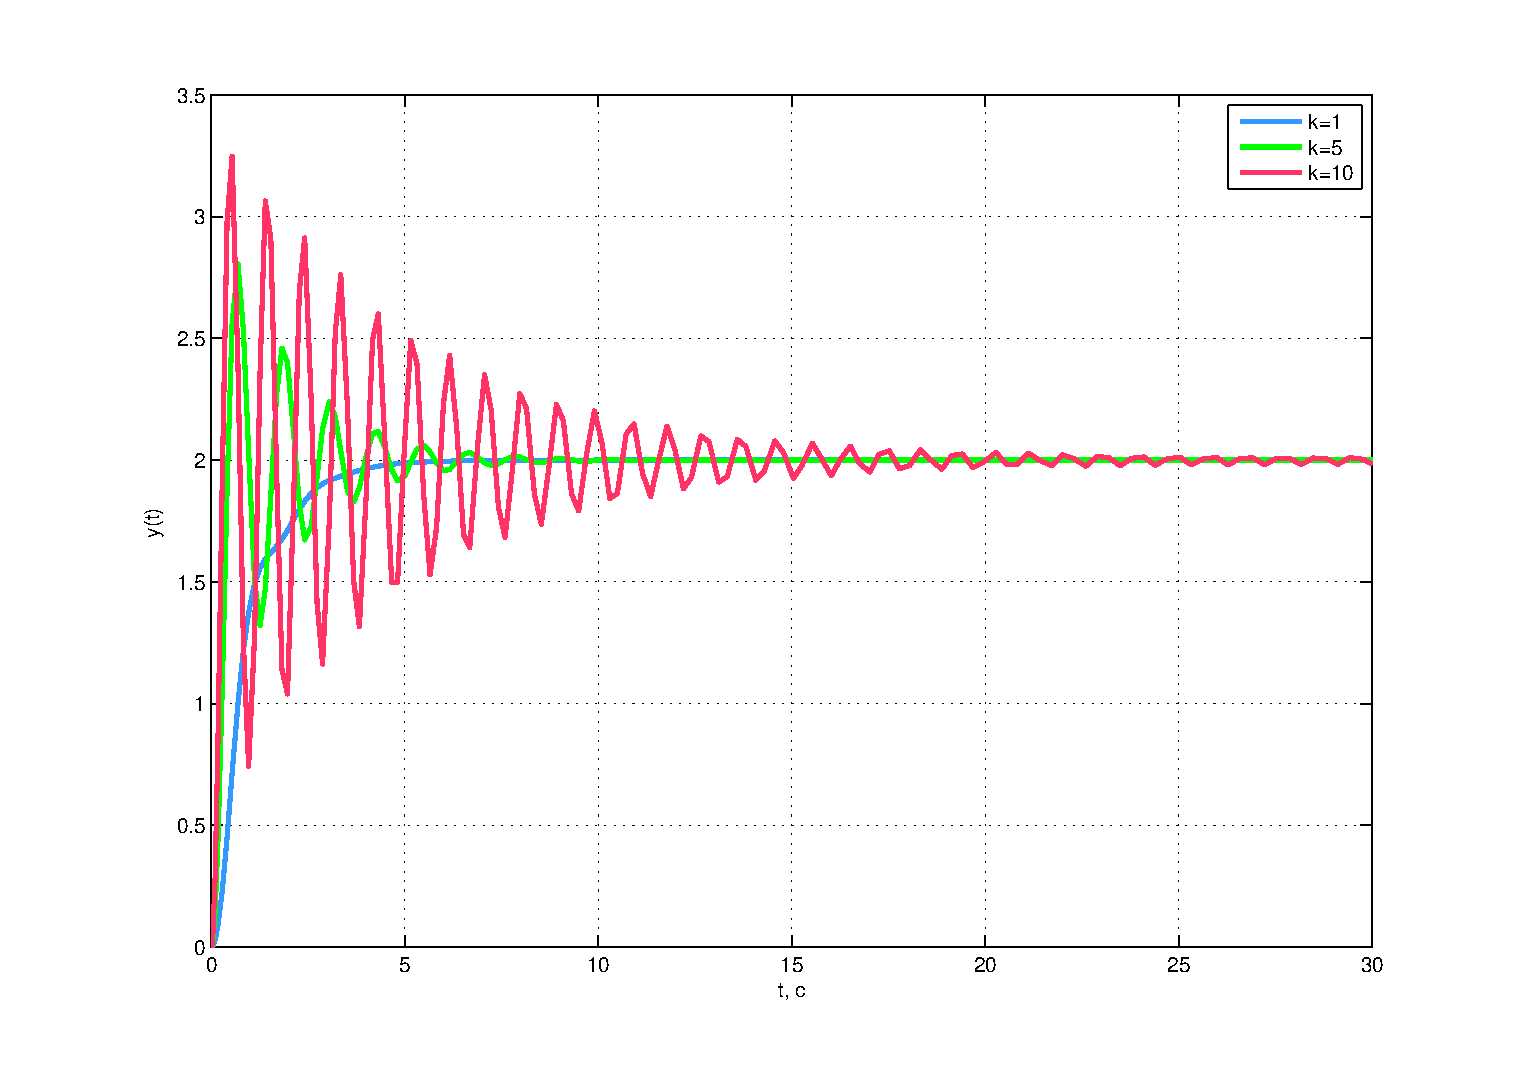
\includegraphics[width=1\linewidth]{scheme/plot5.eps}
	\caption{Переходные характеристики системы для стационарного режима работы}
\end{figure}
\begin{figure}[H]
	\centering
	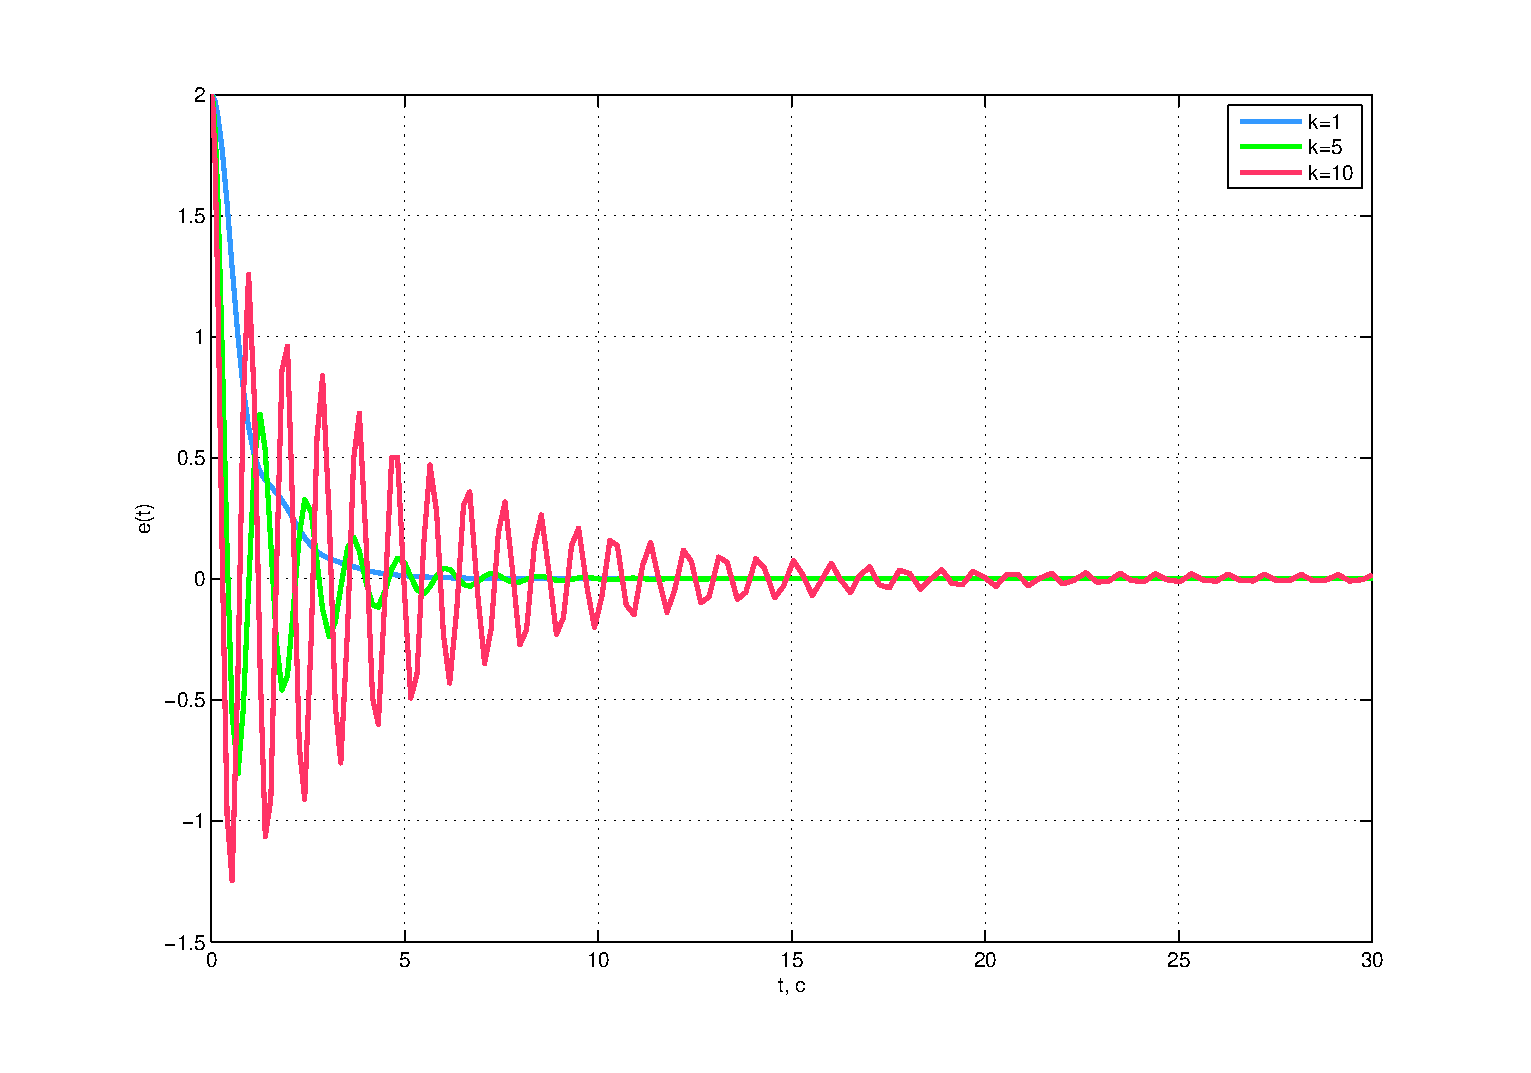
\includegraphics[width=1\linewidth]{scheme/plot6.eps}
	\caption{Переходные характеристики для ошибки}
\end{figure}

\subsection{Исследование режима движения с постоянной скоростью: \\$g(t)=Vt$} 
На рисунке 9 представлена переходная характеристика системы при входном воздействии $g=t$, на рисунке 10  - переходные характеристики для ошибки.
\begin{figure}[H]
	\centering
	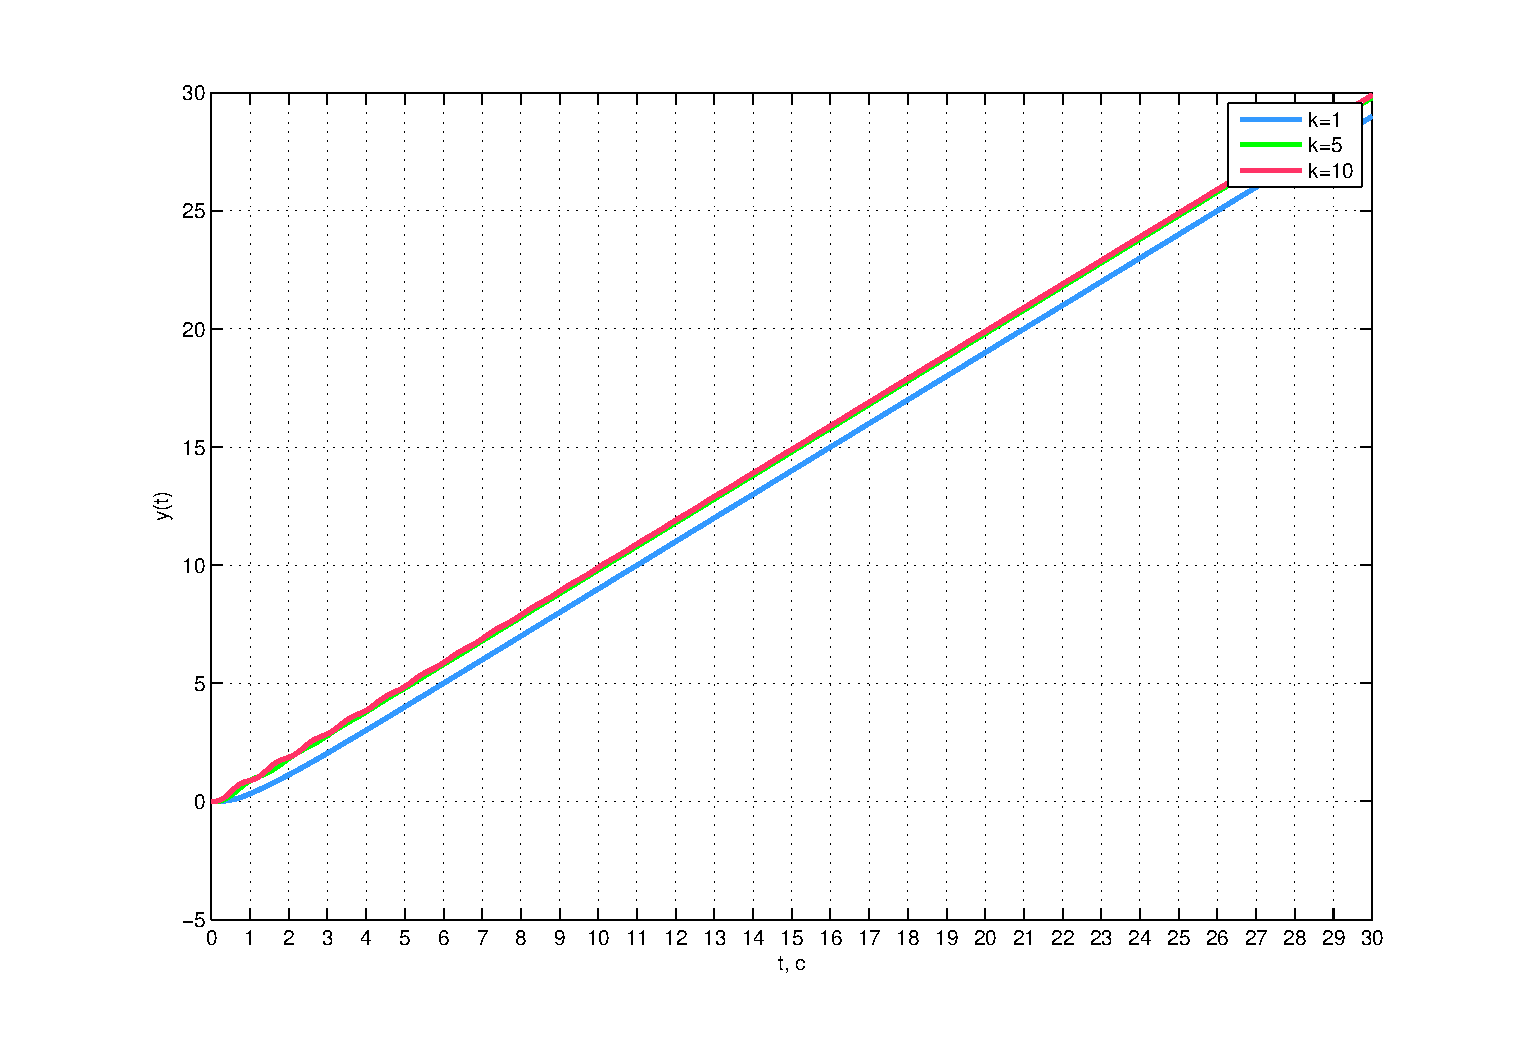
\includegraphics[width=1\linewidth]{scheme/plot7.eps}
	\caption{Переходные характеристики системы для движения с постоянной скоростью}
\end{figure}
При линейно нарастающем воздействии $g(t)=Vt$ предельное значение установившейся ошибки будет равно:
\begin{equation}
    \varepsilon = \lim_{s\to 0}s\frac{1}{1+W(s)}*\frac{V}{s^2} = \lim_{s\to 0}\frac{s}{s+k}\frac{V}{s} = \frac{V}{k}.
\end{equation}
Тогда при $k=1$: $\varepsilon = \displaystyle{\frac{1}{1} = 1;}$\\
при $k=5$: $\varepsilon = \displaystyle{\frac{1}{5} = 0.2;}$\\
при $k=10$: $\varepsilon = \displaystyle{\frac{1}{10} = 0.1}$
\begin{figure}[H]
	\centering
	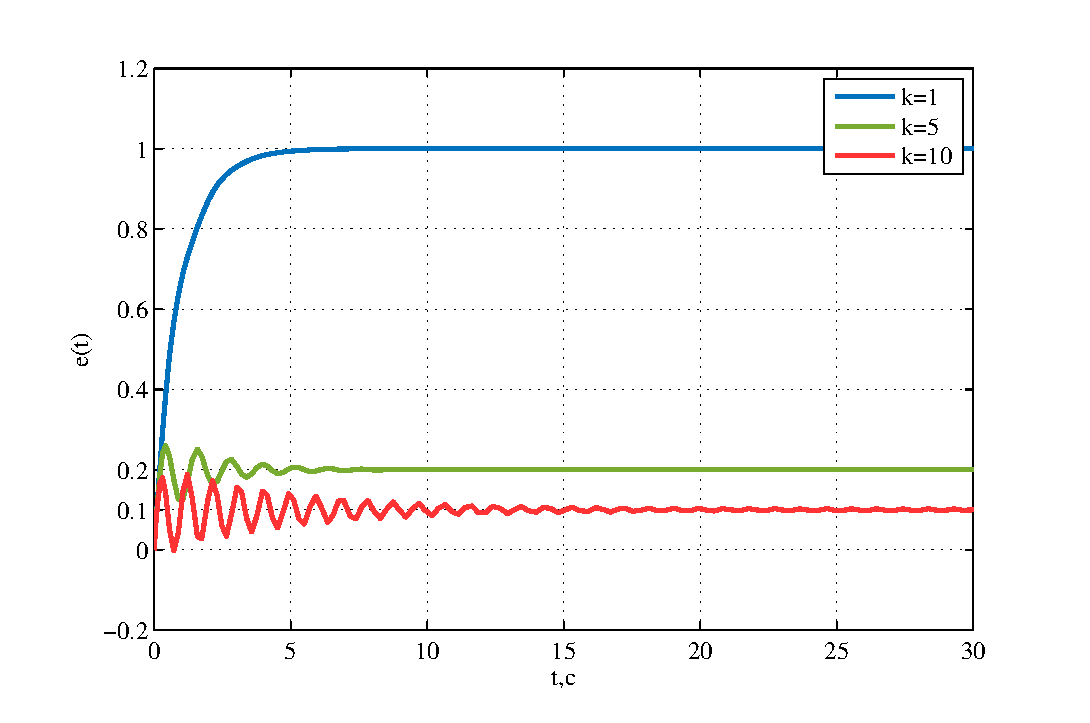
\includegraphics[width=1\linewidth]{scheme/plot8.eps}
	\caption{Переходные характеристики для ошибки}
\end{figure}

\subsection{Исследование режима движения с постоянным ускорением: \\$g(t)=at^2/2$} 
На рисунке 11 представлена переходная характеристика системы при входном воздействии $g=0.3t^2$ и ошибка на рисунке 12.
\begin{figure}[H]
	\centering
	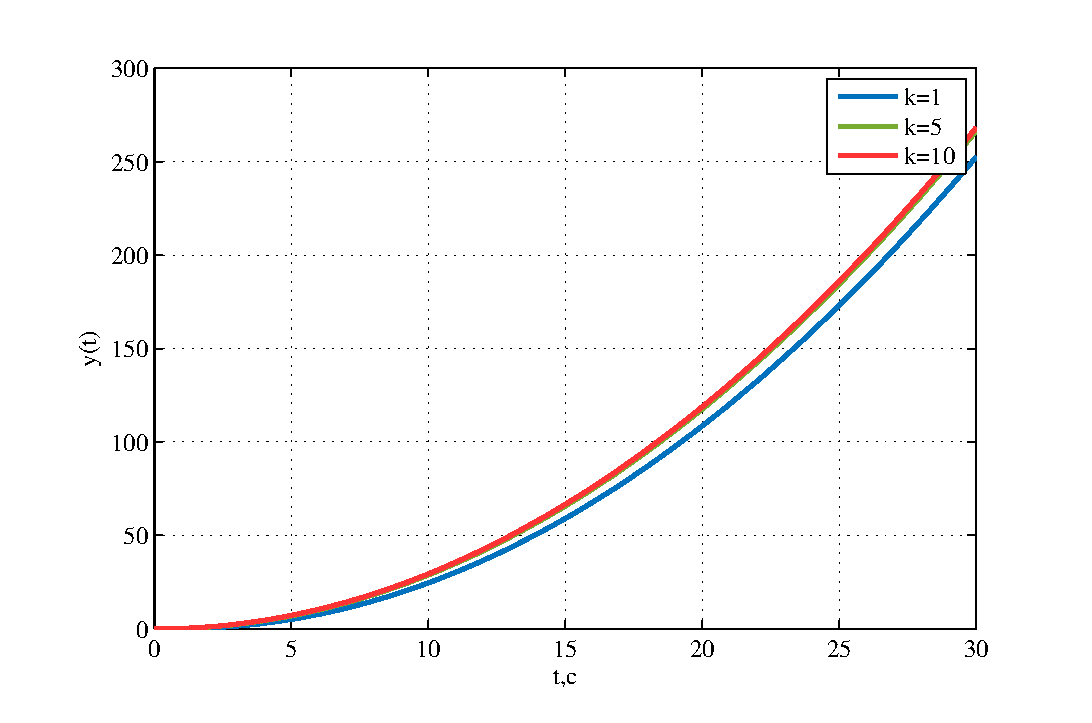
\includegraphics[width=1\linewidth]{scheme/plot9.eps}
	\caption{Переходные характеристики системы для движения с постоянным ускорением}
\end{figure}
\begin{figure}[H]
	\centering
	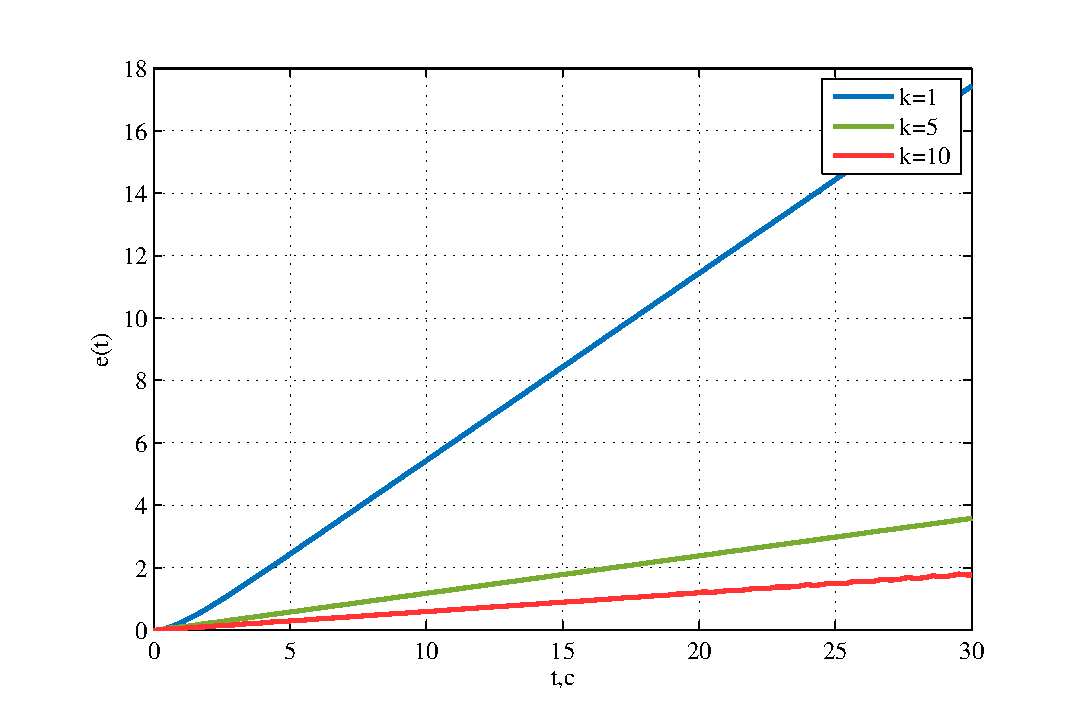
\includegraphics[width=1\linewidth]{scheme/plot10.eps}
	\caption{Переходные характеристики для ошибки при входном воздействии $g=0.3t^2$}
\end{figure}
\par Вывод: в СУ с астатизмом первого порядка ошибка бесконечна.
\newpage
\begin{center}
\section{Исследование влияний внешних возмущений}
\end{center}\par
Структурная схема возмущённой системы при входном воздействии $g=1$ представлена на рисунке 13, также представлены графики переходных процессов (рисунок 14) и переходные характеристики ошибок (рисунок 15) при различных значениях $k$.
\begin{figure}[H]
    \centering
    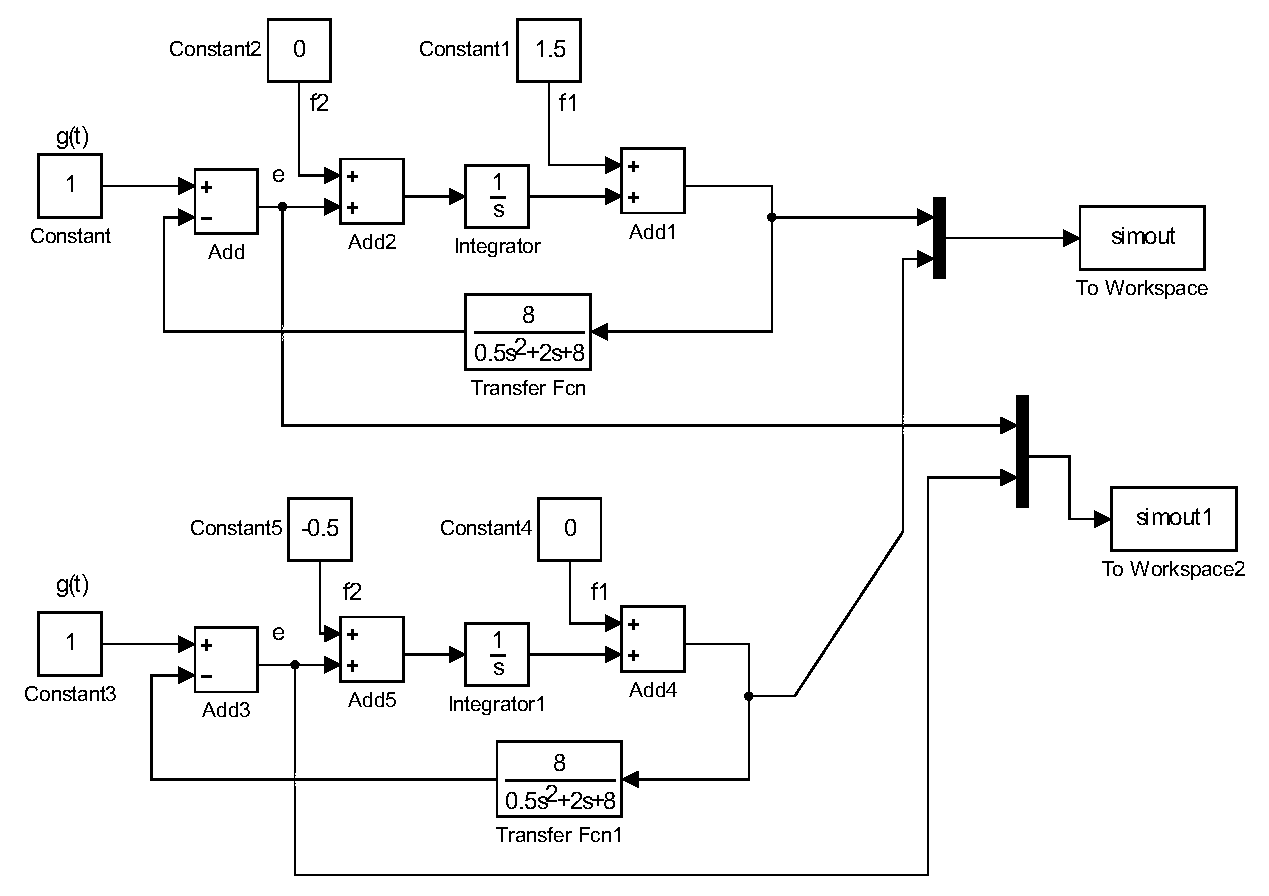
\includegraphics[width=1\linewidth]{scheme/scheme4.eps}
    \caption{Структурная схема системы при влиянии внешних возмущений}
\end{figure}
Функция ошибки слежения равна
\begin{equation}
e = {\frac{g - W(s)f_1 - \displaystyle{\frac{1}{s}}W(s)f_2}{1 + \displaystyle{\frac{1}{s}}W(s)}}=-f_2,
\end{equation}

Положим, что $f_2=0$, тогда предельное значение ошибки при заданных параметрах должно быть равно 0. Если положить  $f_1=0$, тогда предельное значение ошибки будет равно $-f_2$, то есть 0.5.
\begin{figure}[H]
    \centering
    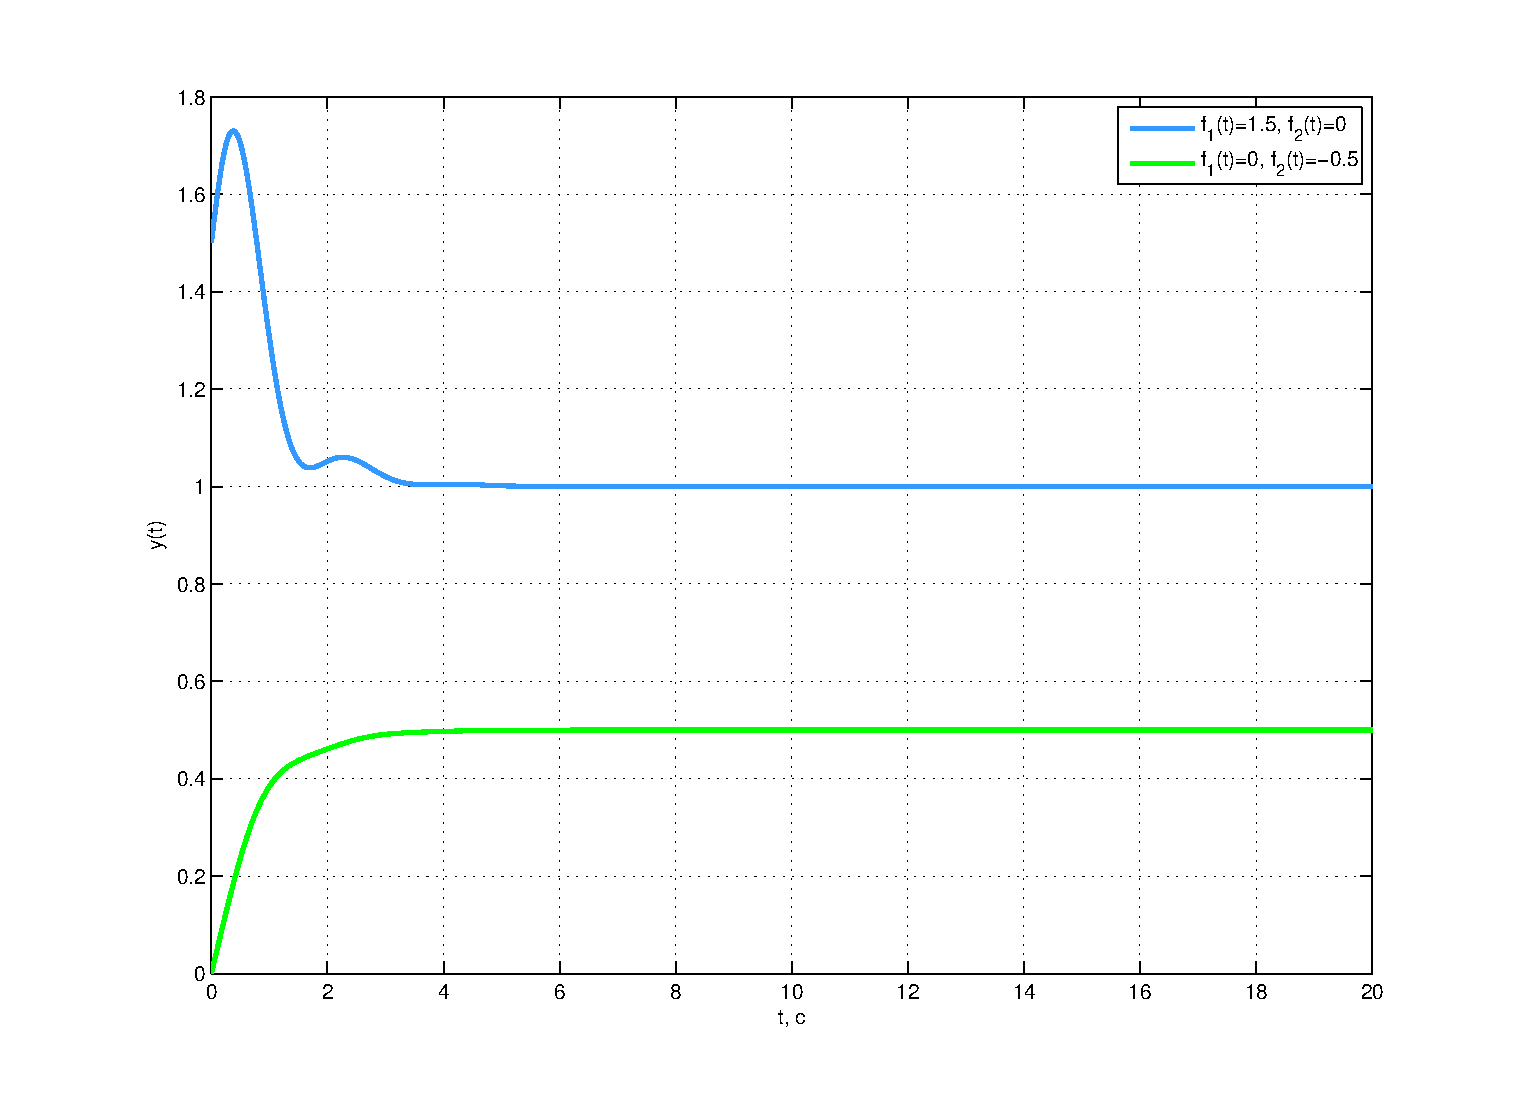
\includegraphics[width=1\linewidth]{scheme/plot11y.eps}
    \caption{Переходные характеристики системы при влиянии внешних возмущений}
\end{figure}
\begin{figure}[H]
    \centering
    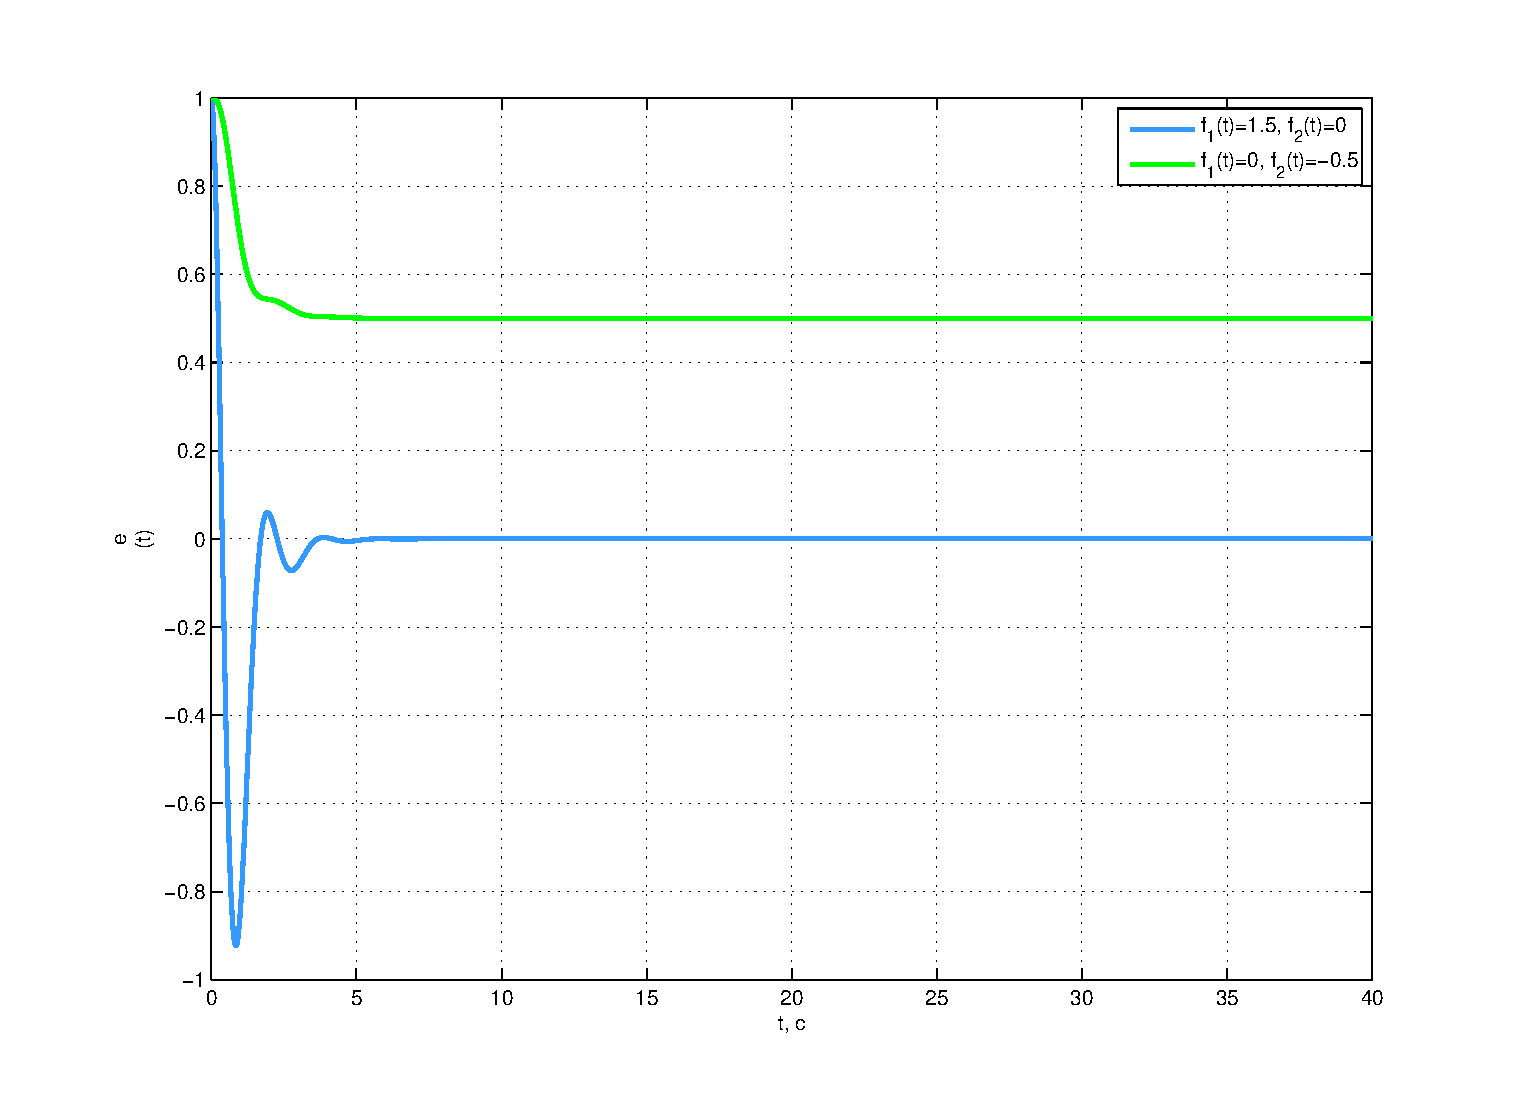
\includegraphics[width=1\linewidth]{scheme/plot12e.eps}
    \caption{Переходные характеристики для ошибки}
\end{figure}

\newpage
\begin{center}
\section{Исследование установившейся ошибки при произвольном входном воздействии}
\end{center}\par
 Структурная схема представлена на рисунке 1, где $H(s) = 1, W(s) = \displaystyle{\frac{8}{0,5s^2 + 2s + 8}}$, а задающее воздействие $g(t) = {5 + t}$.
 В ходе моделирования заданной системы (рисунок 15) был получен график переходного процесса, представленный на рисунке 16. Из него видно, что предельное значение ошибки стремится к $\infty$. Схема моделирования системы представленна на рисунке 13.
\begin{figure}[H]
    \centering
    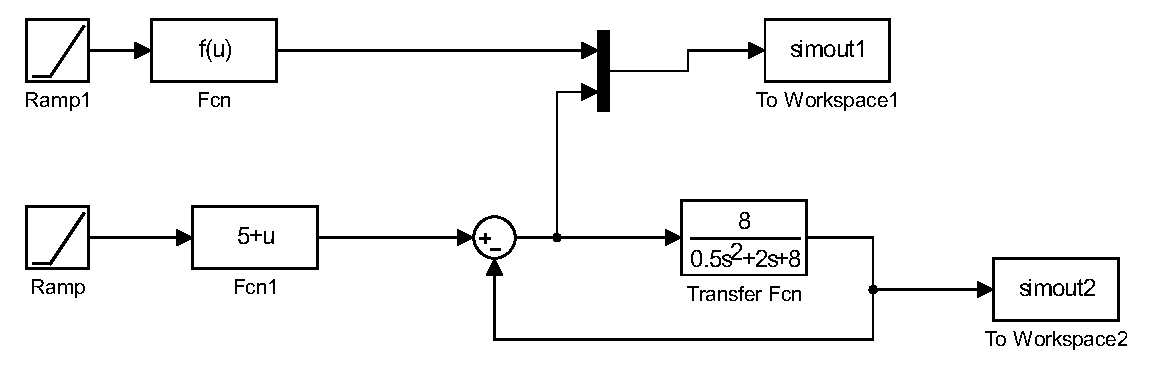
\includegraphics[width=1\linewidth]{scheme/scheme5.eps}
    \caption{Структурная схема системы при произвольном входном воздействии}
\end{figure}
\begin{figure}[H]
    \centering
    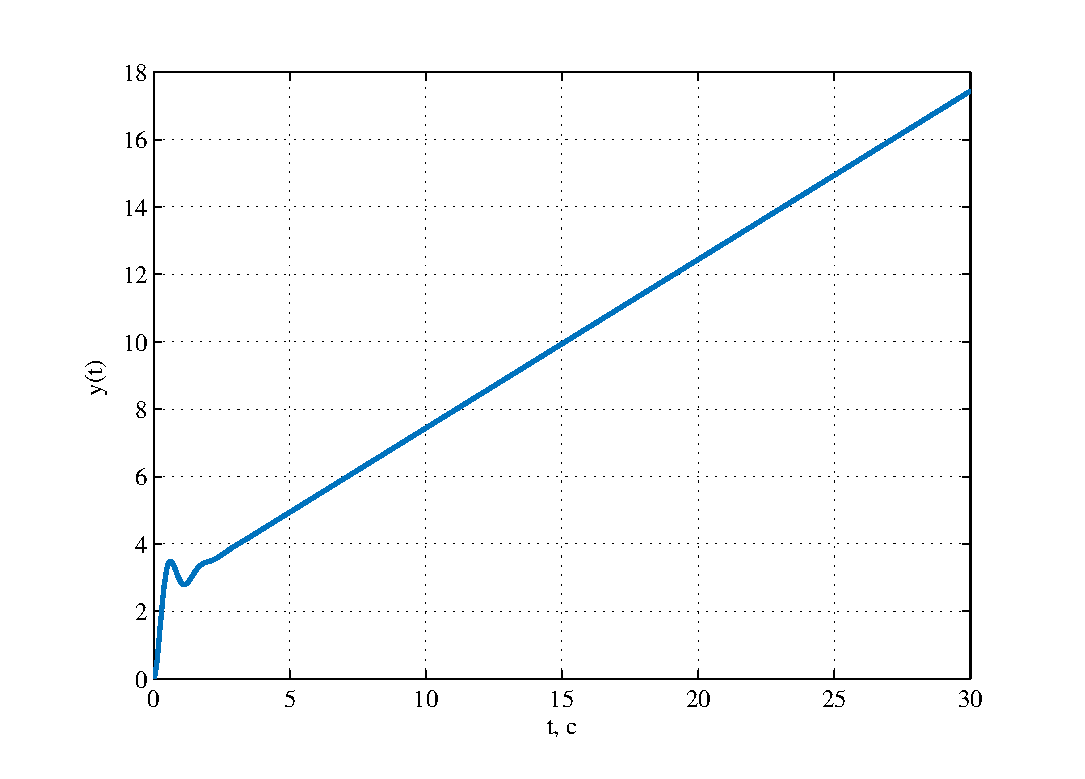
\includegraphics[width=1\linewidth]{scheme/plot13y.eps}
    \caption{Переходной процесс в замкнутой системе при произвольном входном воздействии}
\end{figure}
Получим приближенное аналитическое выражение для установившейся ошибки слежения путём разложения в ряд Тейлора передаточную функцию замкнутой системы по ошибке слежения.
Передаточная функция замкнутой системы по ошибке слежения выглядит так:
\begin{equation}
   \Phi_e(s) = \frac{1}{1 + W(s)} = \frac{1}{1 + \displaystyle{\frac{8}{0,5s^2 + 2s + 8}}} = \frac{0.5s^2 + 2s + 8}{0.5s^2 + 2s + 16}.
\end{equation}\par
При произвольном входном воздействии выражение установившейся ошибки будет выглядеть следующим образом:
\begin{equation}
    e_y(t) = \Phi_e(s)|_{s=0}g(t) + \left.\frac{d\Phi_e(s)}{ds}\right|_{s=0}\dot{g}(t) + \left.\frac{d^2\Phi_e(s)}{ds^2}\right|_{s=0}\frac{\ddot{g}(t)}{2!}.
\end{equation}\par
Найдём производные $g(t)$ и $\Phi_e(s)$:
\begin{align*}
    g(t) & = {t + 5} & \Phi_e(s)|_{s=0} & = \frac{0.5s^2 + 2s + 8}{0.5s^2 + 2s + 16} = 0.5 \\
    \dot{g}(t) & = 1 & \frac{d\Phi_e(s)}{ds}\right|_{s=0} & = {0.0625} \\
    \ddot{g}(t) & = {0} & \\
\end{align*}
\par
Тогда получаем выражение ошибки $e_y(t)$:
\begin{equation}
e_y(t) = {0.5(t + 5) + 0.0625 * 1 + 0} = 0.5t + 2.5625.
\end{equation}\par
Убедимся, что графики расчетной и экспериментально определённой установившейся ошибки слежения совпадают для этого построим их на одном графике, представленном на рисунке 17.
\begin{figure}[H]
    \centering
    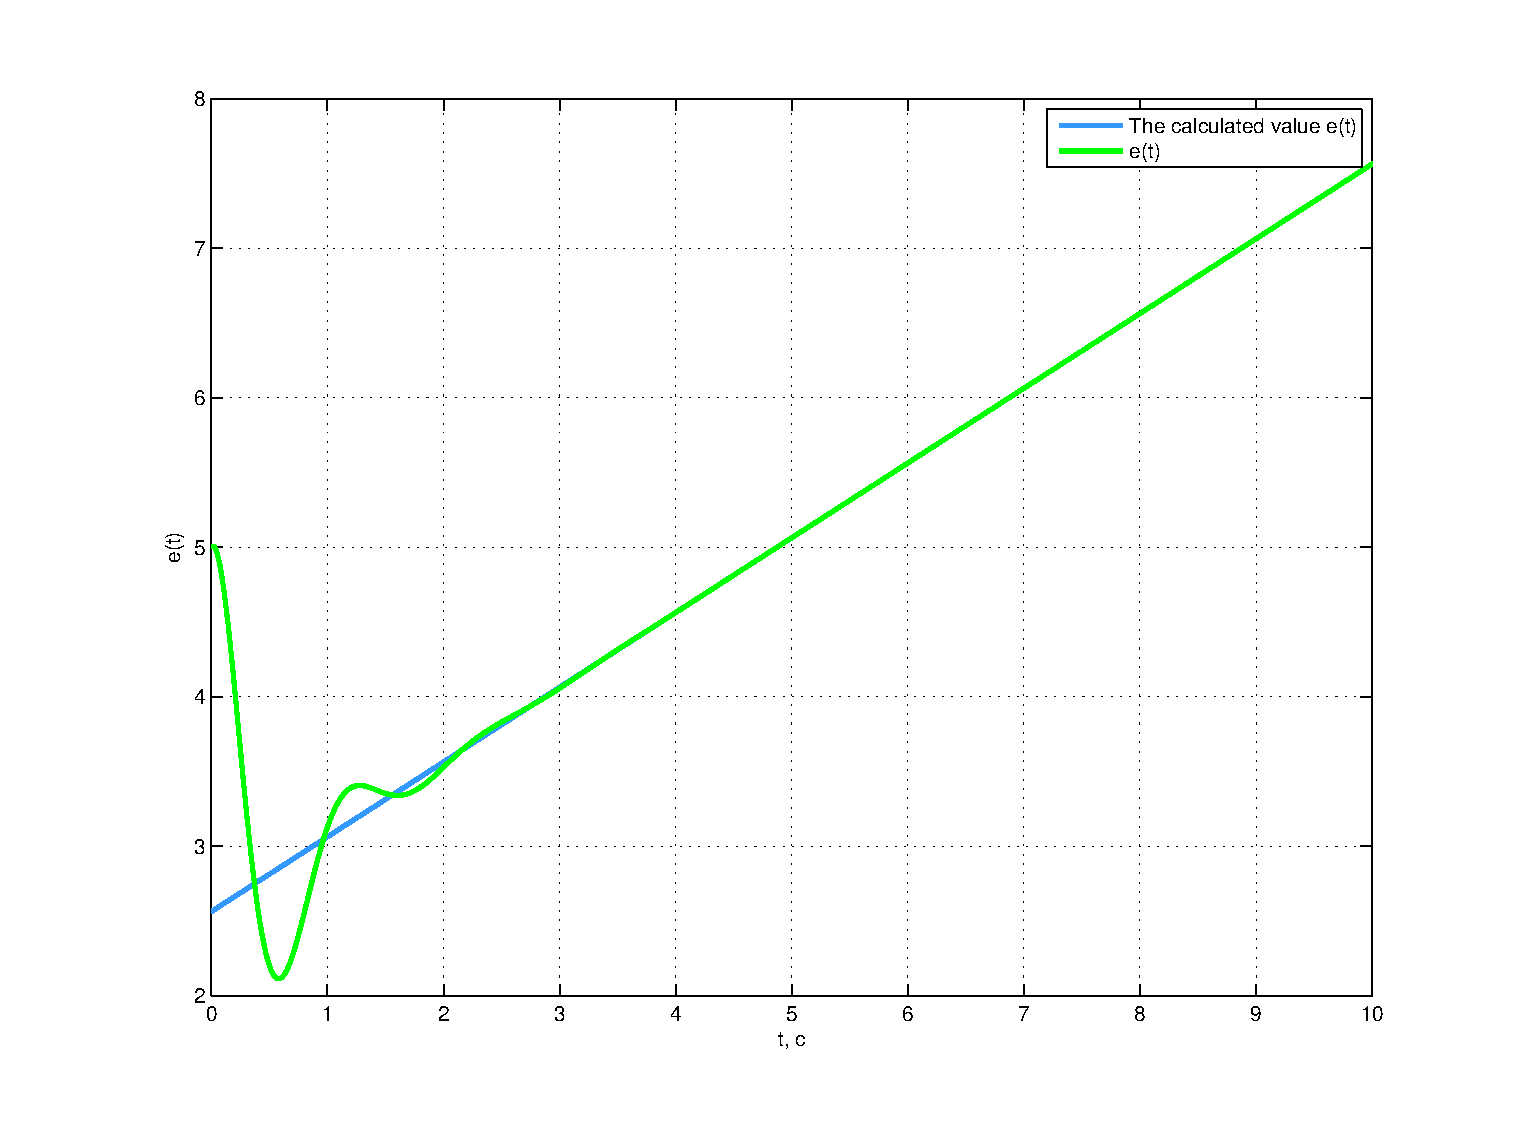
\includegraphics[width=1\linewidth]{scheme/plot14e.eps}
    \caption{Графики ошибок}
\end{figure}

\newpage
\begin{center}
\section{Вывод}
\end{center}
\par
В ходе лабораторной работы были исследованы системы с разным порядком астатизма, при влиянии внешних возмущений и при произвольном входном воздействии. Были построены переходные характеристики для всех случаев и найдены значения установившихся ошибок. Данные исследования позволяют сделать вывод о том что, установившееся значение ошибки можно изменить путём увеличения или уменьшения общего коэффициента усиления разомкнутой системы, а также путём снижения или повышения порядка астатизма.Кроме того было показано, что порядок астатизма системы по задающему воздействию, в общем случае, не соответствует порядку астатизма по возмущению.Так же было получено приближенное аналитическое выражение для установившейся ошибки слежения системы при произвольном входном воздействии.


\end{document}